\chapter{Performance tests}\label{S:Performance-Test}
In this chapter the results for a GPIO performance tests are shown. This tests will be done using the Raspberry Pi and two implementations of IOSharp, the original written in C\# which has been explained on the first part of this thesis, the second implementation tested will be the C++ one translated from the original by AlterNative which has been explained in the second part of this thesis. Theoretically, C++ has a major performance compared to C\# but this tests are used to determine how much the C++ implementation gains over the C\# ones.
\\
To make the measures in this tests the Logic16 has been used. This is a channel analyzer used to record, view, and measure digital signals. It also currently has 17 different protocol analyzers including SPI, serial, I2C and many more.

\section{Compilation types}\label{S:PERF-comptypes}
When a compiler generates a binary from a source code normally tries to do some changes to optimize the some attributes of the program. The most common requirement is to optimize the time taken to execute that program, another one is optimize the amount of memory required, also some optimizations can be used to make a program consume less power and this is interesting because nowadays smartphones and tablets have a small battery so reaching low power consumption is great to have long battery life. All of this optimizations are carried out by a sequence of optimizing transformations and algorithms high help create programs that uses fewer resources.
\\
Normally compilers can generate programs using optimizations or without using them. If the compiler uses optimizations the compile time will growth but the program will be much more optimized than if the compiler does not apply them.
\begin{itemize}
  \item \textbf{Non-optimized or debug:} this compile mode is used by developers who want to debug applications in execution time. In this case the whole symbol information which is used by the debugger to stop at the break points (designated instructions). For example the .pdb files from Visual Studio are created by the compiler and have the information to debug the created binary. But normally the debug mode will not allow some optimizations because are incompatible to the properly function of the debugger.
  \item \textbf{Optimized or release:} this compile mode is used to generate an optimized binary to execute much faster than the debug one. In this case the compiler performs different transformations to the original code, for example two typical optimizations that cannot be applied to the debug mode are:
  \begin{itemize}
  	\item \textbf{Loop unrolling:} the compiler replaces the code inside a loop (for example inside a for). This helps avoiding the maintenance of the loop variables.
  	\item \textbf{Inlining:} the compiler places the method on the place of the call avoiding the overhead of the calling stack to the method.
  	\begin{lstlisting}[language=C++, caption={Inline example}]
inline int Max(int x, int y)
{
   return (x > y)? x : y;
}
int main( )
{
   int a = 100;
   int b = 1010;
   cout << "Max (a, b): " << Max(100,1010) << endl;
   return 0;
}

/* The Max(int, int) function is inlined to the main Max call in the following way:*/
int main( )
{
   int a = 100;
   int b = 1010;
   cout << "Max (100,1010): " << (a>b)? a : b << endl;
   return 0;
}
\end{lstlisting}
  \end{itemize}
\end{itemize}

\section{GPIO}\label{SS:IOEx-GPIO}
The GPIO test consists on how much time takes the board to perform a certain number of iterations changing an output port between the high and low states. Two channels are used in this test, the first one will activate the Logic to start sniffing the second channel which will be the one that performs the output between the two states.
\\
The code used in this test is shown below, both the original version and the translated one using AlterNative.
\begin{lstlisting}[language=CSharp, caption={GPIO Performance test in C\#}]
using System;
using System.Collections.Generic;
using System.Linq;
using System.Text;
using Microsoft.SPOT.Hardware;
using IOSharp.NETMF.RaspberryPi.Hardware;
using System.Threading;

namespace raspberrypi
{
    class Program
    {
        public static void Main()
        {
            Debug.Print("START");
            OutputPort bar = new OutputPort(Pins.V2_GPIO17, false);
            bar.Write(false);
            bool foo = false;
            OutputPort o = new OutputPort(Pins.V2_GPIO11, false);

            bar.Write(true);
            for (int i = 0; i < 10000; i++)
            {
                foo = !foo;
                o.Write(foo);
            }
            bar.Write(false);
            Debug.Print("END");
        }
    }
}
\end{lstlisting}

\begin{lstlisting}[language=C++, caption={GPIO Performance translated to C++}]
#include "Program.h"
namespace raspberrypi {

	void Program::Main(){
		Program* p = new Program();
		p->Run();
	}

	void Program::Run(){
		Debug::Print(new String("START"));
		OutputPort* bar = new OutputPort(Cpu::Pin::GPIO_Pin17, false);
	
		bar->Write(false);
		bool foo = false;
		OutputPort* o = new OutputPort(Cpu::Pin::GPIO_Pin11, false);
		bar->Write(true);
		for (int i = 0; i < 200; i += 1) {
			Debug::Print(new String(i));
			foo = !foo;
			o->Write(foo);
		}
		bar->Write(false);
		Debug::Print(new String("END"));
	}
}
\end{lstlisting}

This test will be executed varying the number of iterations between 200 and 10000. Each iteration will swap the port between high and low. Apart from the iteration increase, two type of compilations will be done changing the optimization type between quick compilation without optimization (Debug) and with optimizations (Release).

\subsection{200 Iterations}\label{SS:200-iterations}
The result produced by Mono and the binary compiled in release mode (optimized) shows an irregular pattern consisting of two small pulses a wide pulse and then two small pulses followed by wide gap. In the figure \ref{fig:gpio-200it-csharp} this pattern is coloured in blue and as it can be seen it is regularly repeated across all the test. The wide pulses and gaps are supposed to be caused by the garbage collector or the thread round-roving that Mono does.
\\
The small pulses are around 1 ms and the wide gaps/pulses are 2 ms. Each block is repeated every 10 ms.
\begin{figure}[H]\begin{center}
 \centering
  \captionsetup{justification=centering}
  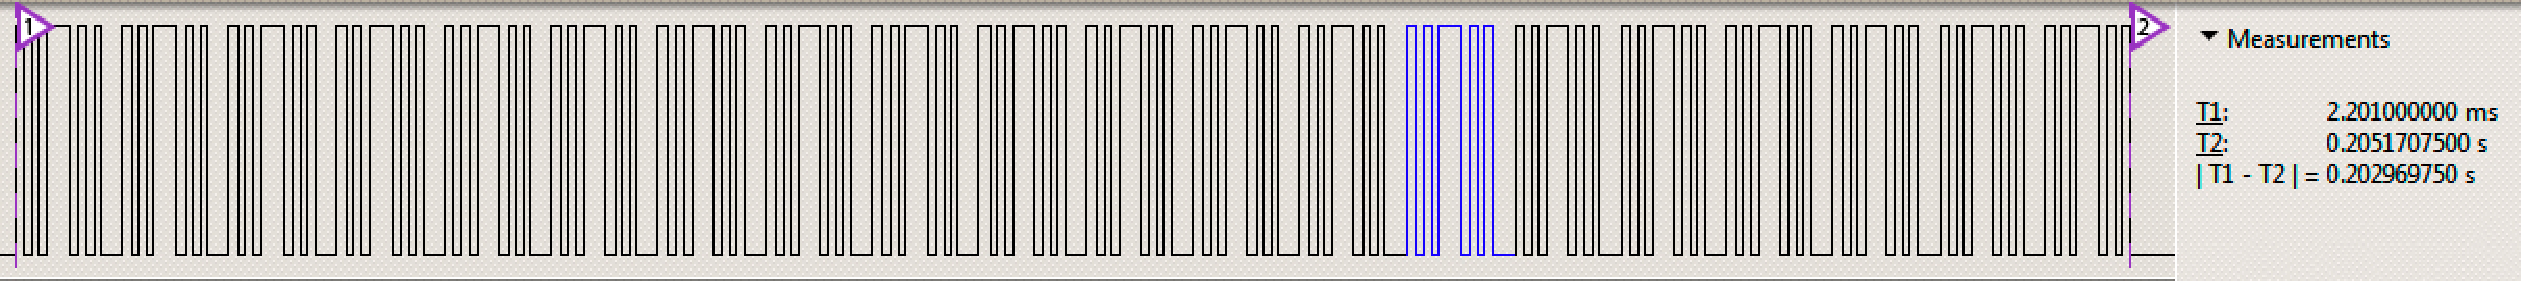
\includegraphics[scale=0.35]{pictures/performance-tests/GPIO/200/csharp2}
  \caption{200 Iterations using C\# with optimizations \label{fig:gpio-200it-csharp}}
\end{center}\end{figure}
The figure \ref{fig:gpio-200it-csharp} represents 200 changes between state high and low in an OutputPort in the Raspberry Pi under Mono. The required time to make this iterations is the elapsed time between the marker 1 and the marker 2. The Raspberry Pi with Mono needs 202 ms in order to do all the iterations.
\\
\\
After testing the performance in Mono it was time to try out the generated code by AlterNative compiled also in release mode. The resulting test is shown and explained below.
\begin{figure}[H]\begin{center}
 \centering
  \captionsetup{justification=centering}
  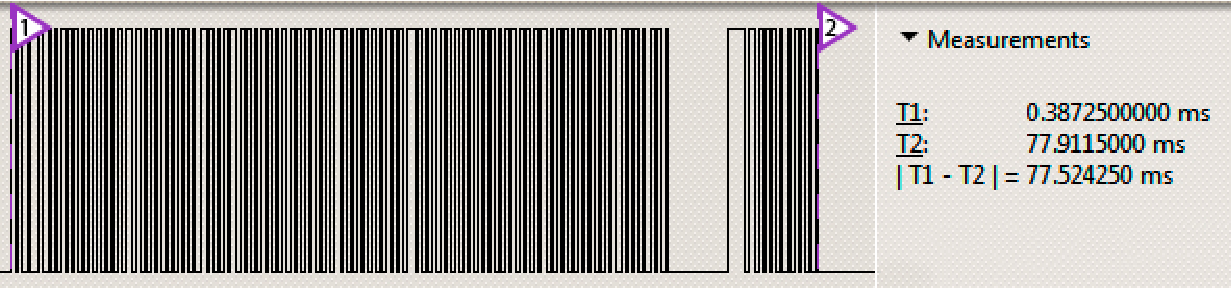
\includegraphics[scale=0.35]{pictures/performance-tests/GPIO/200/cxx}
  \caption{200 Iterations using C++ with optimizations \label{fig:gpio-200it-cxx}}
\end{center}\end{figure}
This image is in the same scale that the C\# one, so the magnitude of the elapsed time can be compared.
In case of C++ test it can be observed that the pulses are much more regular than the mono test, but at certain point around the pulse 89 a big gap is observed probably due to the lack of a garbage collector (AlterNative programs currently do not have a working garbage collector implemented). It is interesting to remark that C++ needs only 77 ms to perform the same test, and each pulse is 0.43 ms on average.
\\
\\
After doing some tests on debug and release mode in both languages a graphic could be sketched, the performance in 200 iterations in Mono using both compile types was the practically the same, it takes around 200 ms to complete all the test, however in C++ the time varies a bit depending on the compilation type, without using optimizations it takes 100 ms but when the compile is done in release mode the time decreases to 78 ms.
\\
From the figure \ref{fig:gpio-graph-200} it can be concluded that the C++ version is a 62\% faster than the Mono version.
\begin{figure}[H]\begin{center}
 \centering
  \captionsetup{justification=centering}
  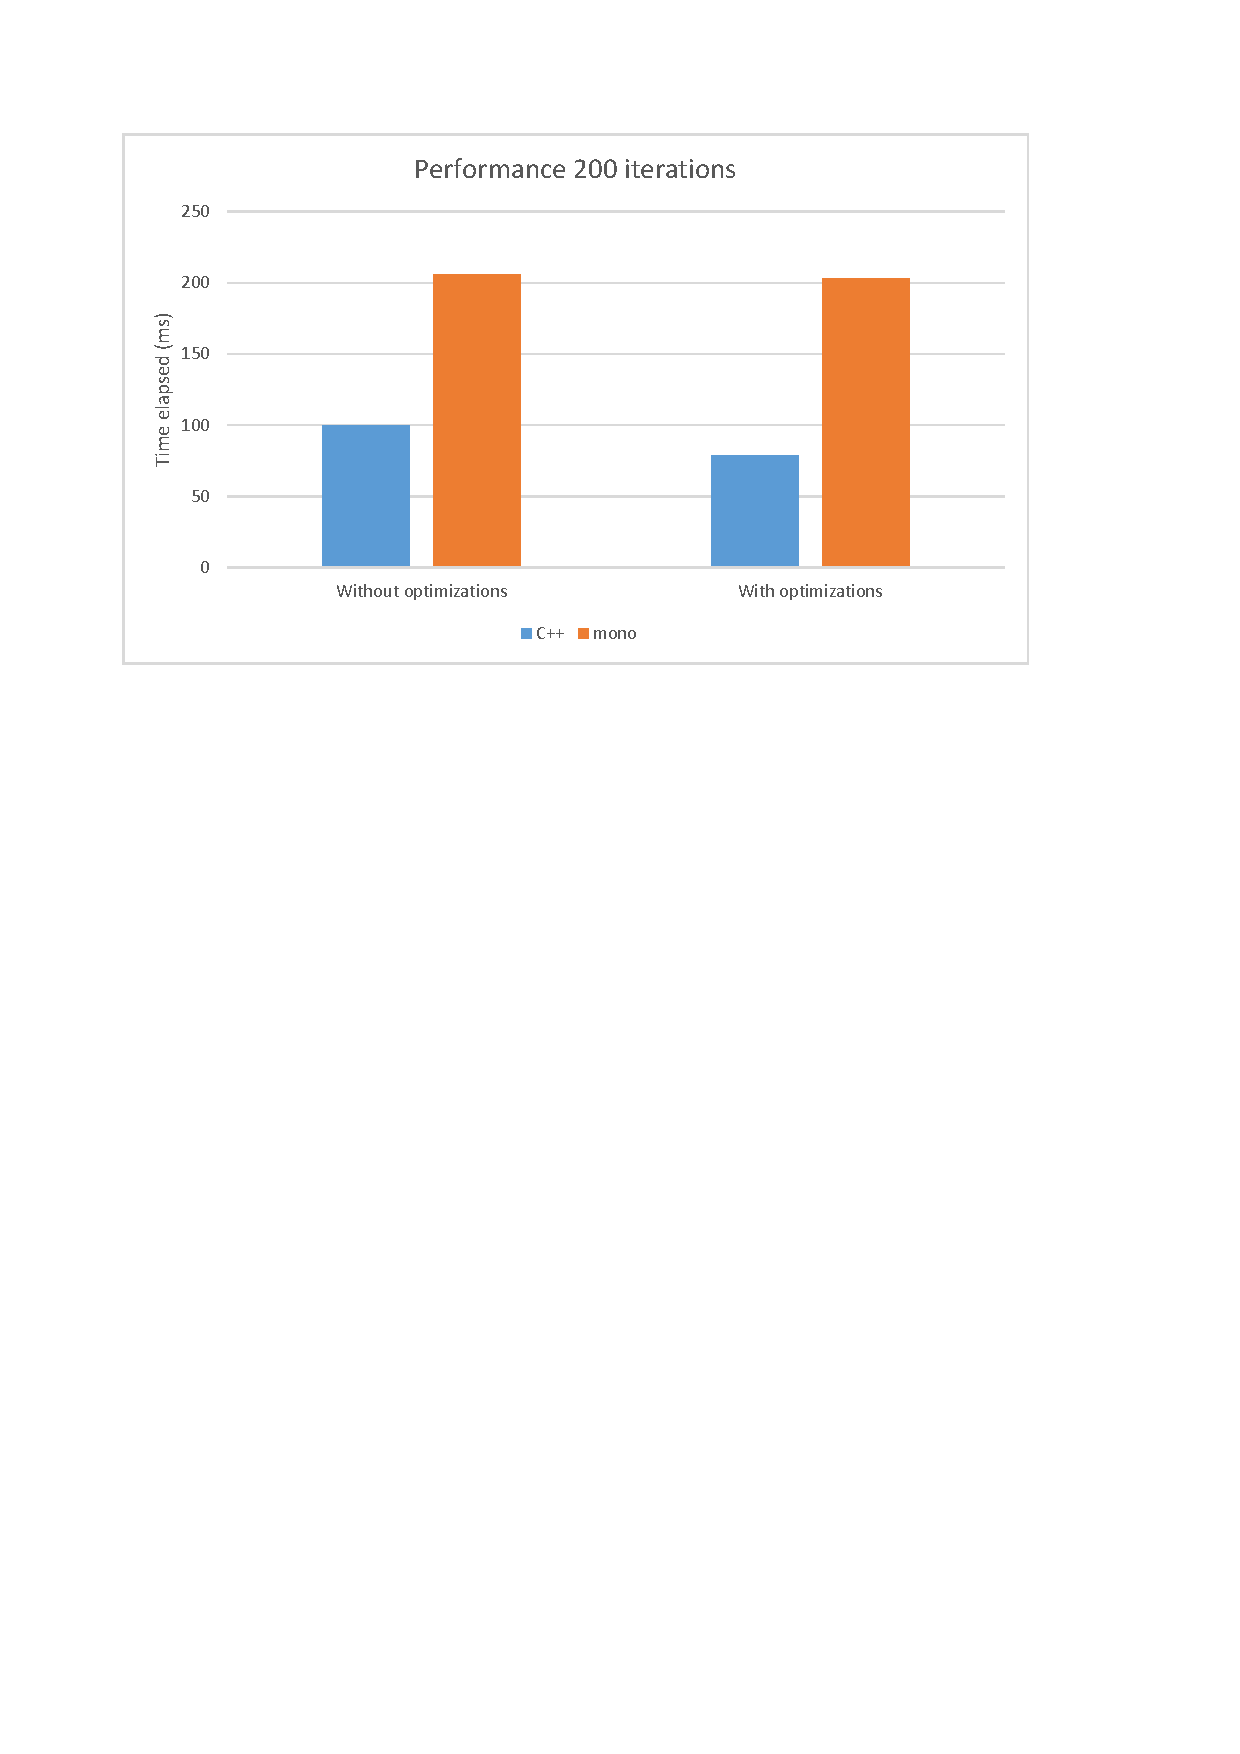
\includegraphics[scale=0.9,page=1]{pictures/performance-tests/GPIO/graphs}
  \caption{Graph showing the elapsed time for the 200 iteration test. Blue is for C++ while orange is C\#. On the left is represented the non-optimized compilations and on the right the optimized ones\label{fig:gpio-graph-200}}
\end{center}\end{figure}

\subsection{10K Iterations}\label{SS:10K-iterations}
After the first test using 200 iterations another one was done, but this time increasing to 10000 iterations or a factor of fifty, in this magnitude the compiler optimizations should be visible enough to observe some kind of improvement on the different compilation types.
\begin{figure}[H]\begin{center}
 \centering
  \captionsetup{justification=centering}
  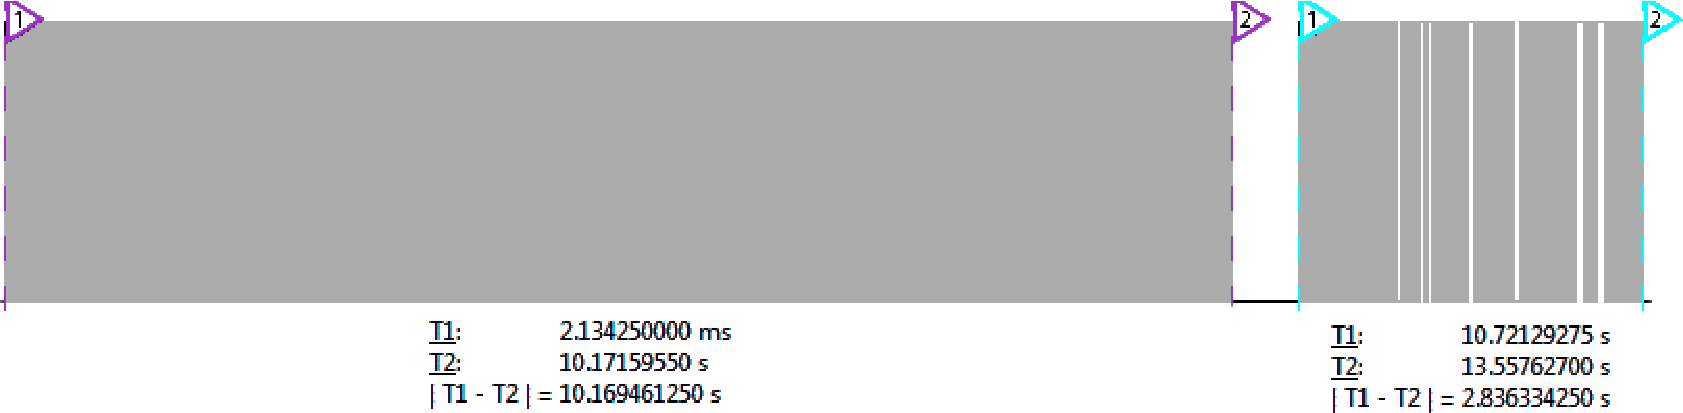
\includegraphics[width=1\textwidth]{pictures/performance-tests/GPIO/10k/cxx+csharp}
  \caption{200 Iterations using C\# with optimizations \label{fig:gpio-200it-csharp}}
\end{center}\end{figure}
\begin{figure}[H]\begin{center}
 \centering
  \captionsetup{justification=centering}
  \includegraphics[scale=0.9,page=2]{pictures/performance-tests/GPIO/graphs}
  \caption{Graph showing the elapsed time for the 10k iteration test. Blue is for C++ while orange is C\#. On the left is represented the non-optimized compilations and on the right the optimized ones\label{fig:gpio-graph-10k}}
\end{center}\end{figure}

\section{Interruptions}\label{SS:IOEx-Interruptions}
It was observed that in HomeSense the response time between sensor events was poor, probably because of the time that mono takes between an interruption is detected to the instructions from the program are executed. To analyze this an interruption test was done to know how much time passes between the trigger and the result. So in this case the program will start and wait until an event occurs on a GPIO, then another GPIO will be set to an output port and change its state to high, this will be the measured time.
\\
